\chapter{Results and Analysis}
This chapter presents the experimental results for the proposed speech enhancement system. The performance of the MetricGAN-based method is evaluated and compared with the classical Wiener filter baseline, using both objective and perceptual speech quality metrics.

For the reference the figure representing original signal without noise is depicted below:
\begin{figure}[H]
    \centering
    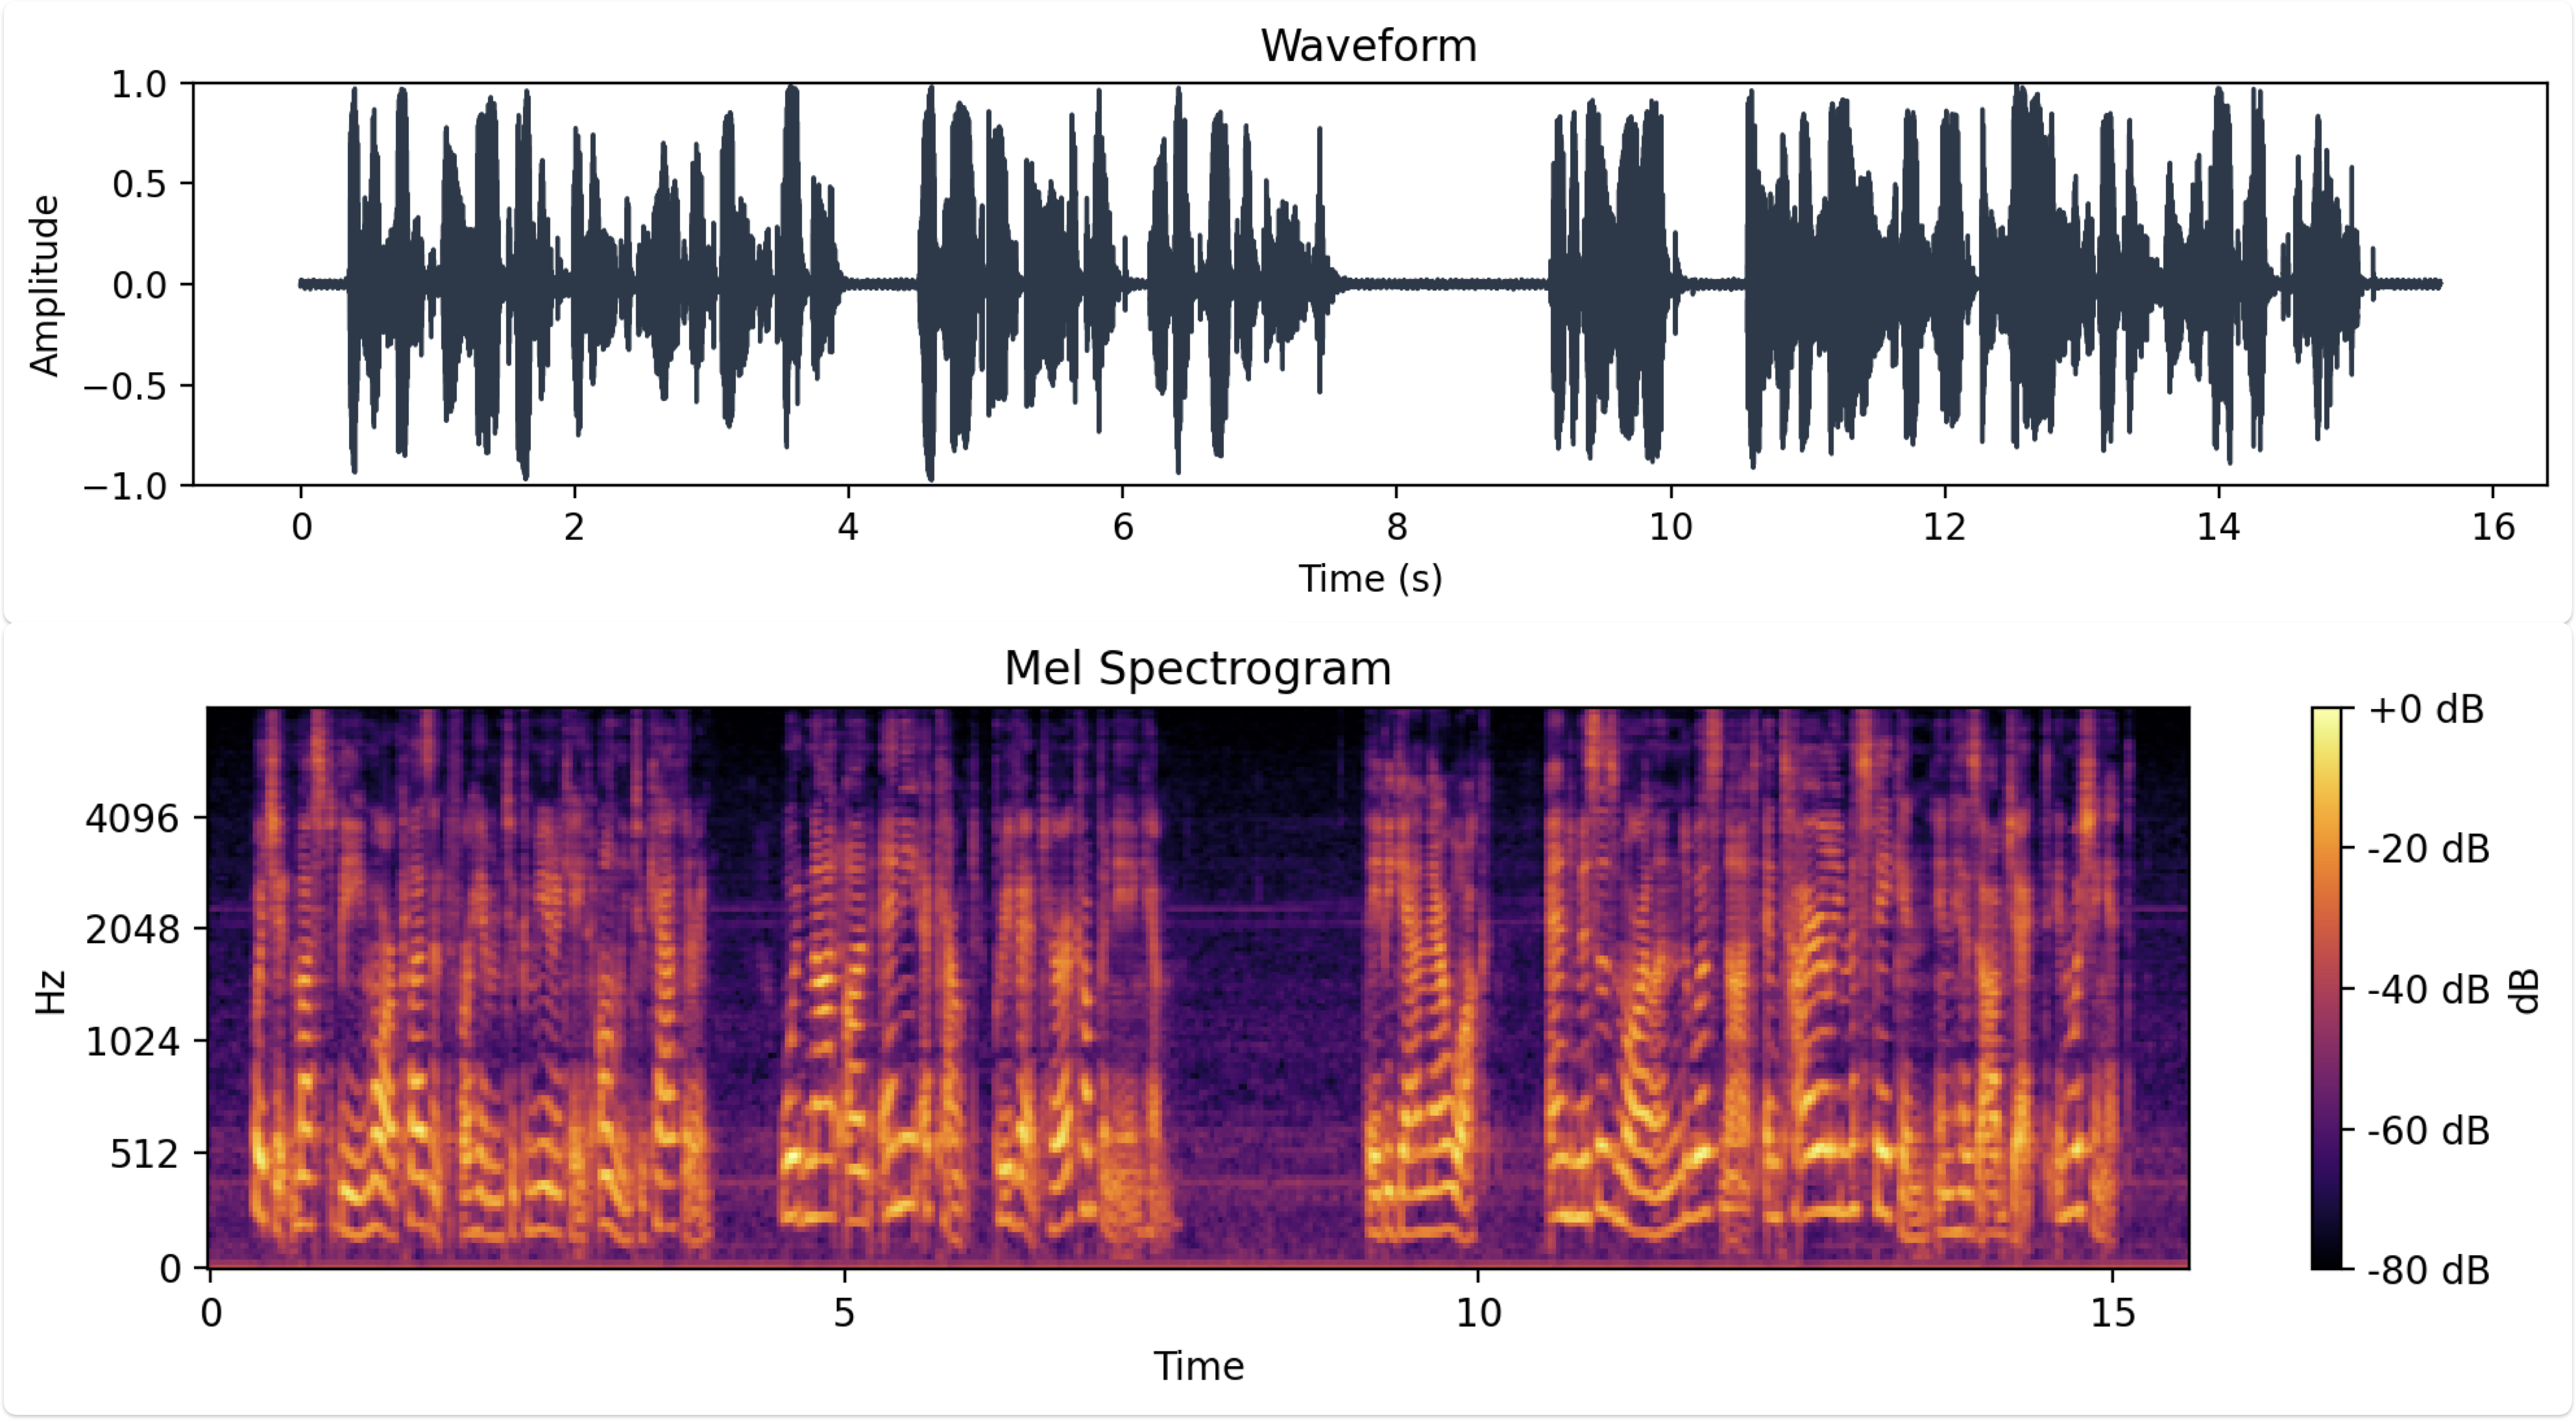
\includegraphics[width=.7\linewidth]{figures/original_.png}
     \caption{Original speech signal waveform}
    \label{fig:figure8}
\end{figure}



Sample was taken from LibriSpeech. Audio was affected by white noise with  0, 5, 10, 15, 20 SNR values. 


\begin{figure}[H]
    \centering
         \begin{subfigure}[b]{0.3\textwidth}
             \centering
             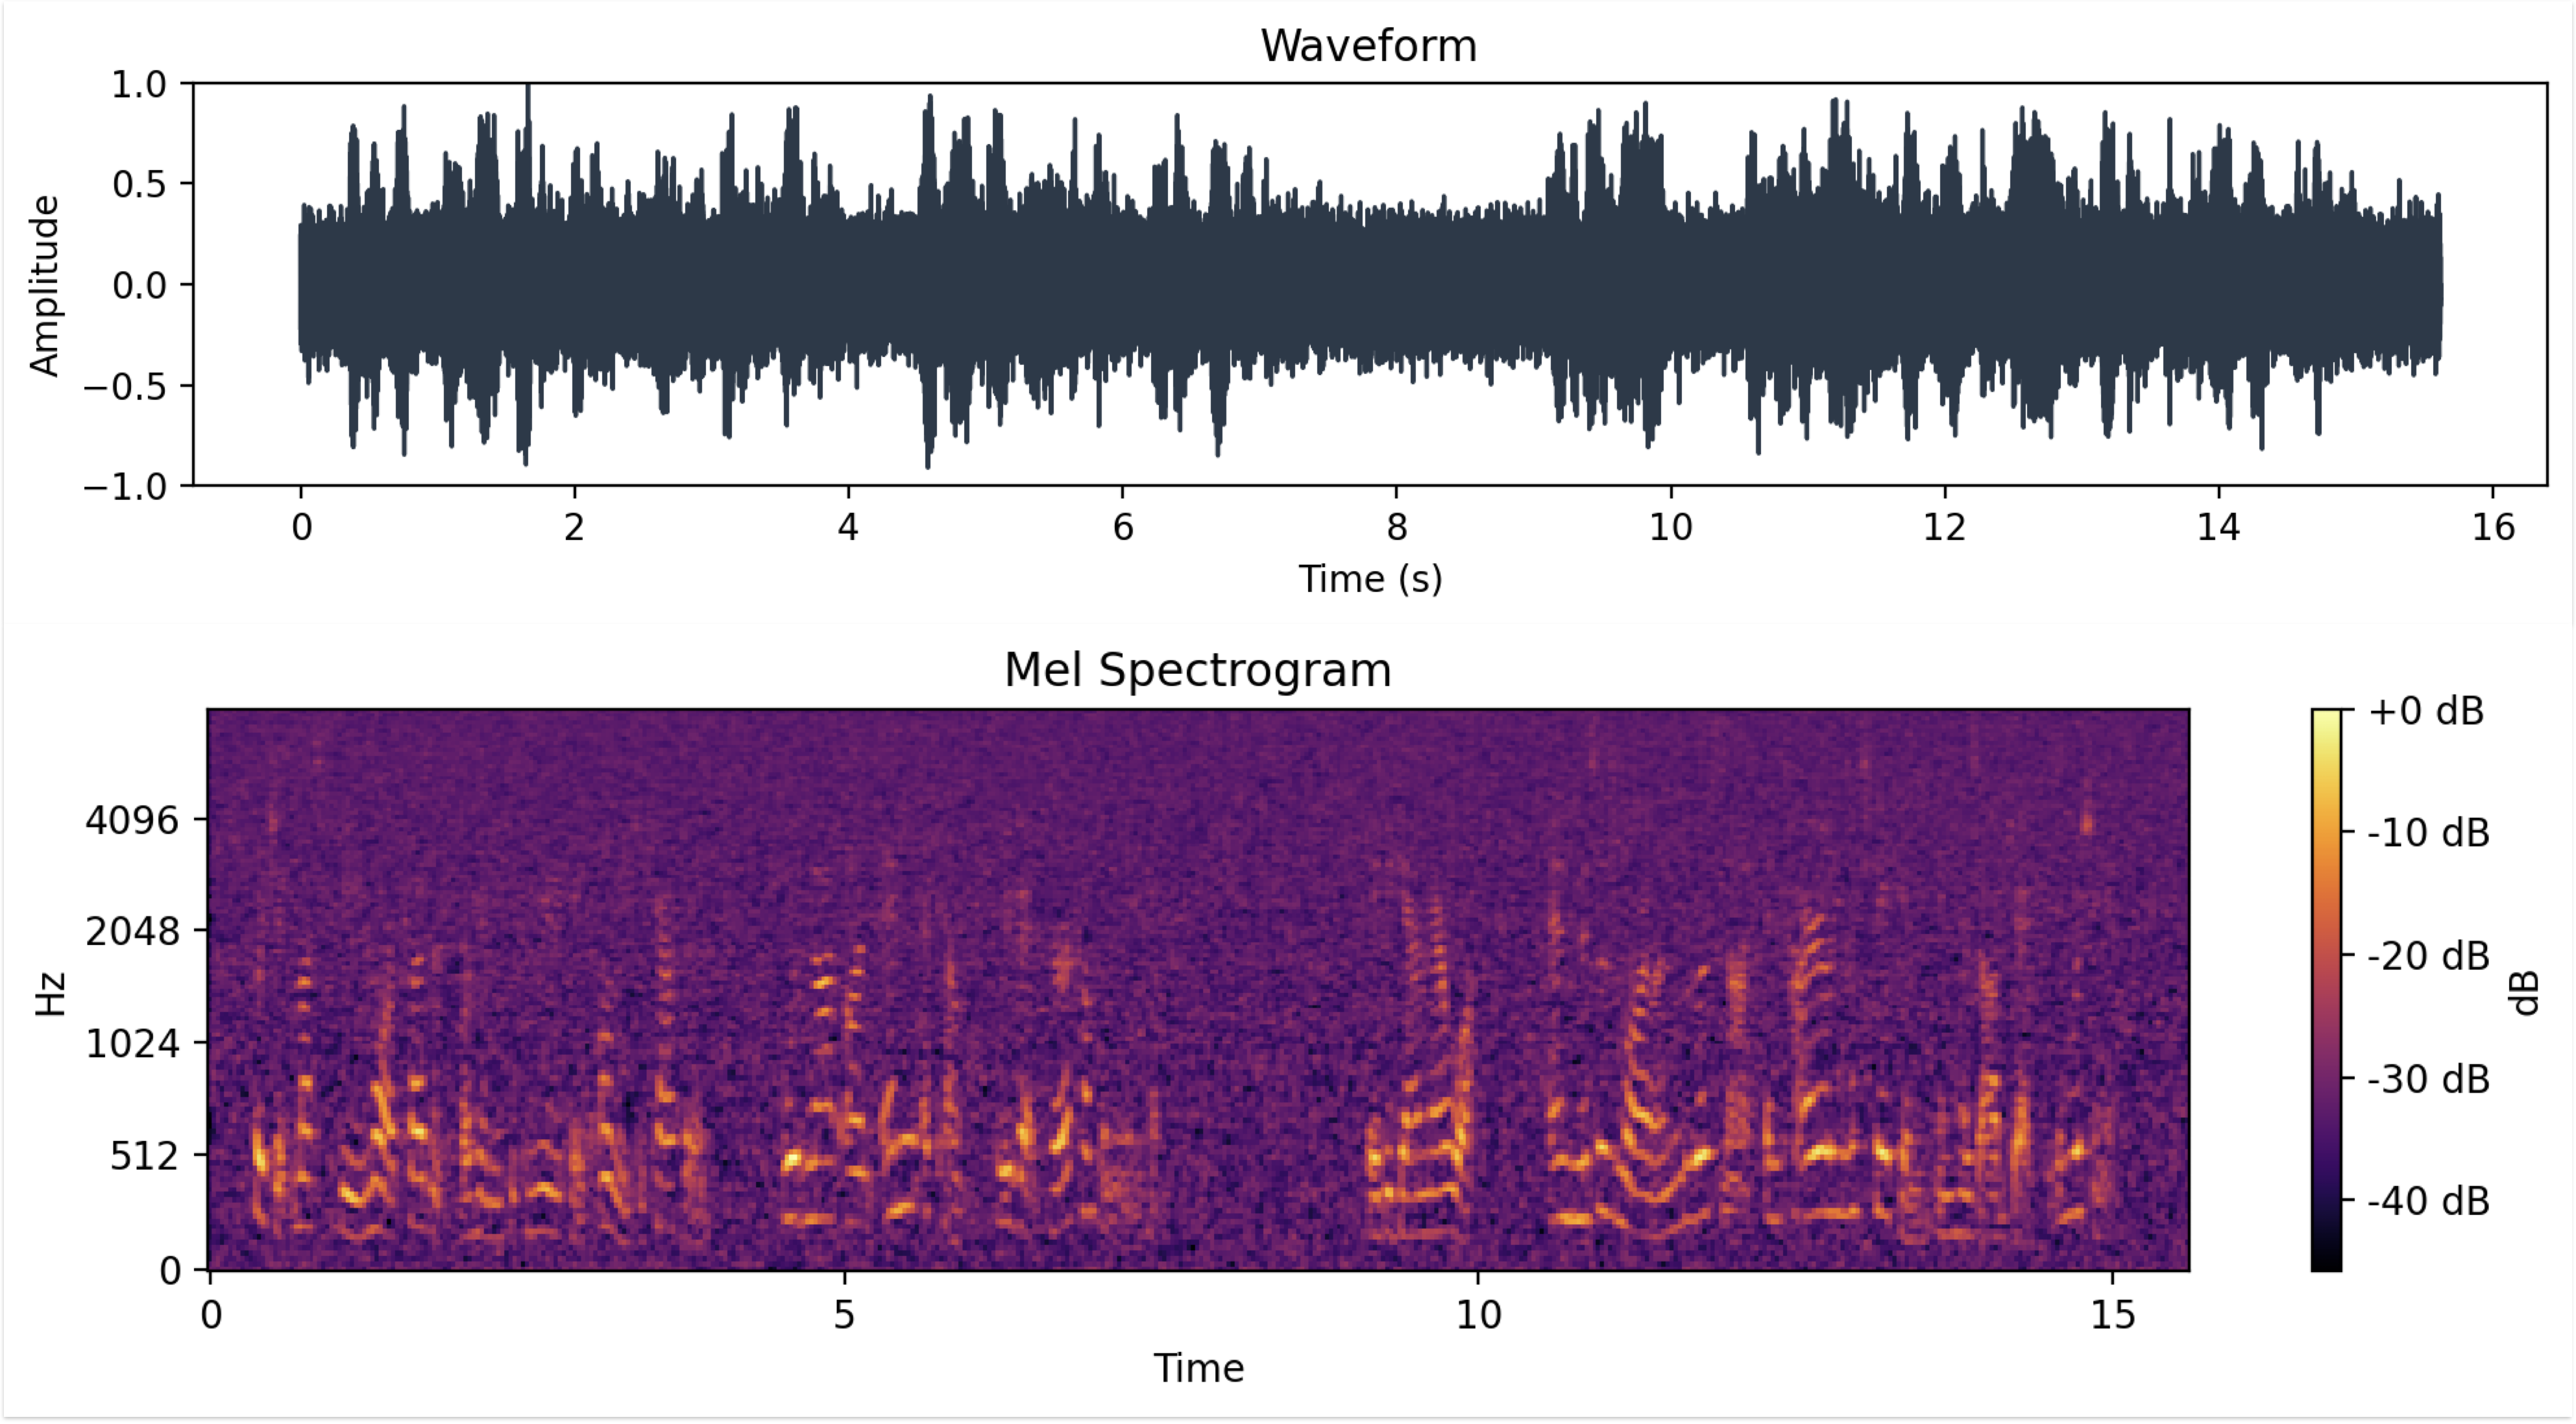
\includegraphics[width=\textwidth]{figures/snr0_o.png}
             \caption{Noisy Speech Signal}
             \label{fig:y equals x}
         \end{subfigure}
         \hfill
         \begin{subfigure}[b]{0.3\textwidth}
             \centering
             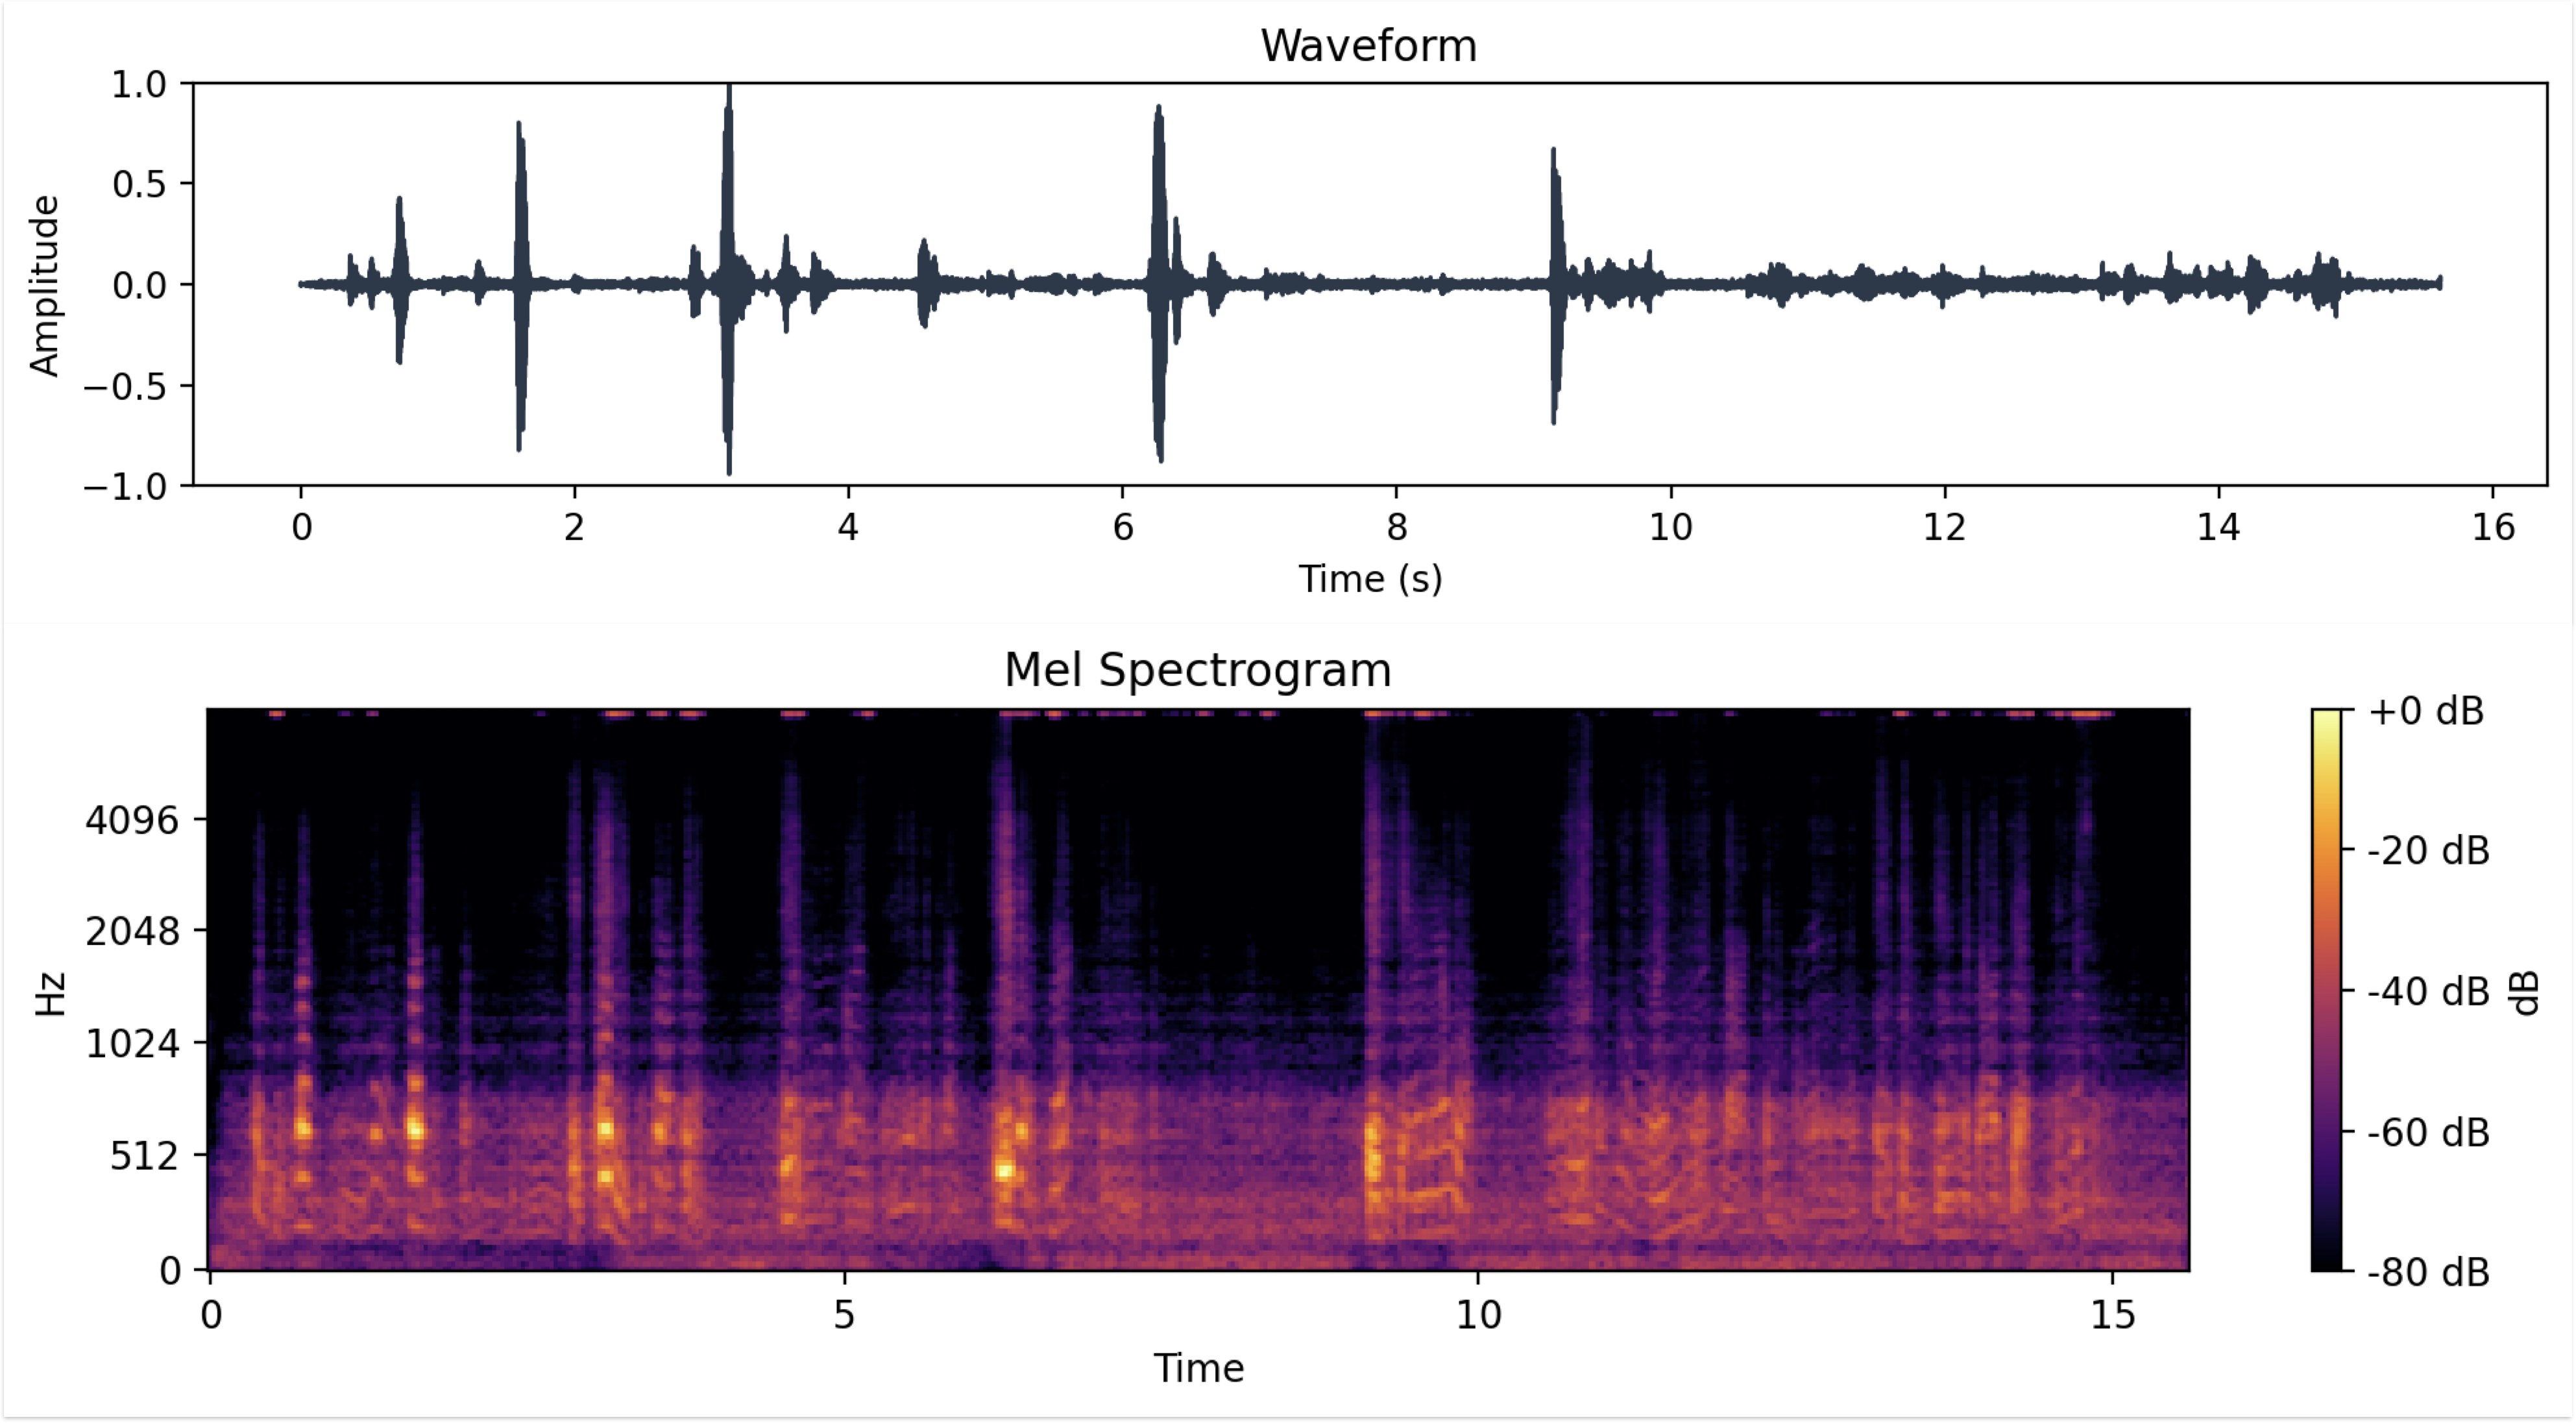
\includegraphics[width=\textwidth]{figures/snr0_e.png}
             \caption{MetricGAN Enhancement}
             \label{fig:three sin x}
         \end{subfigure}
         \hfill
         \begin{subfigure}[b]{0.3\textwidth}
             \centering
             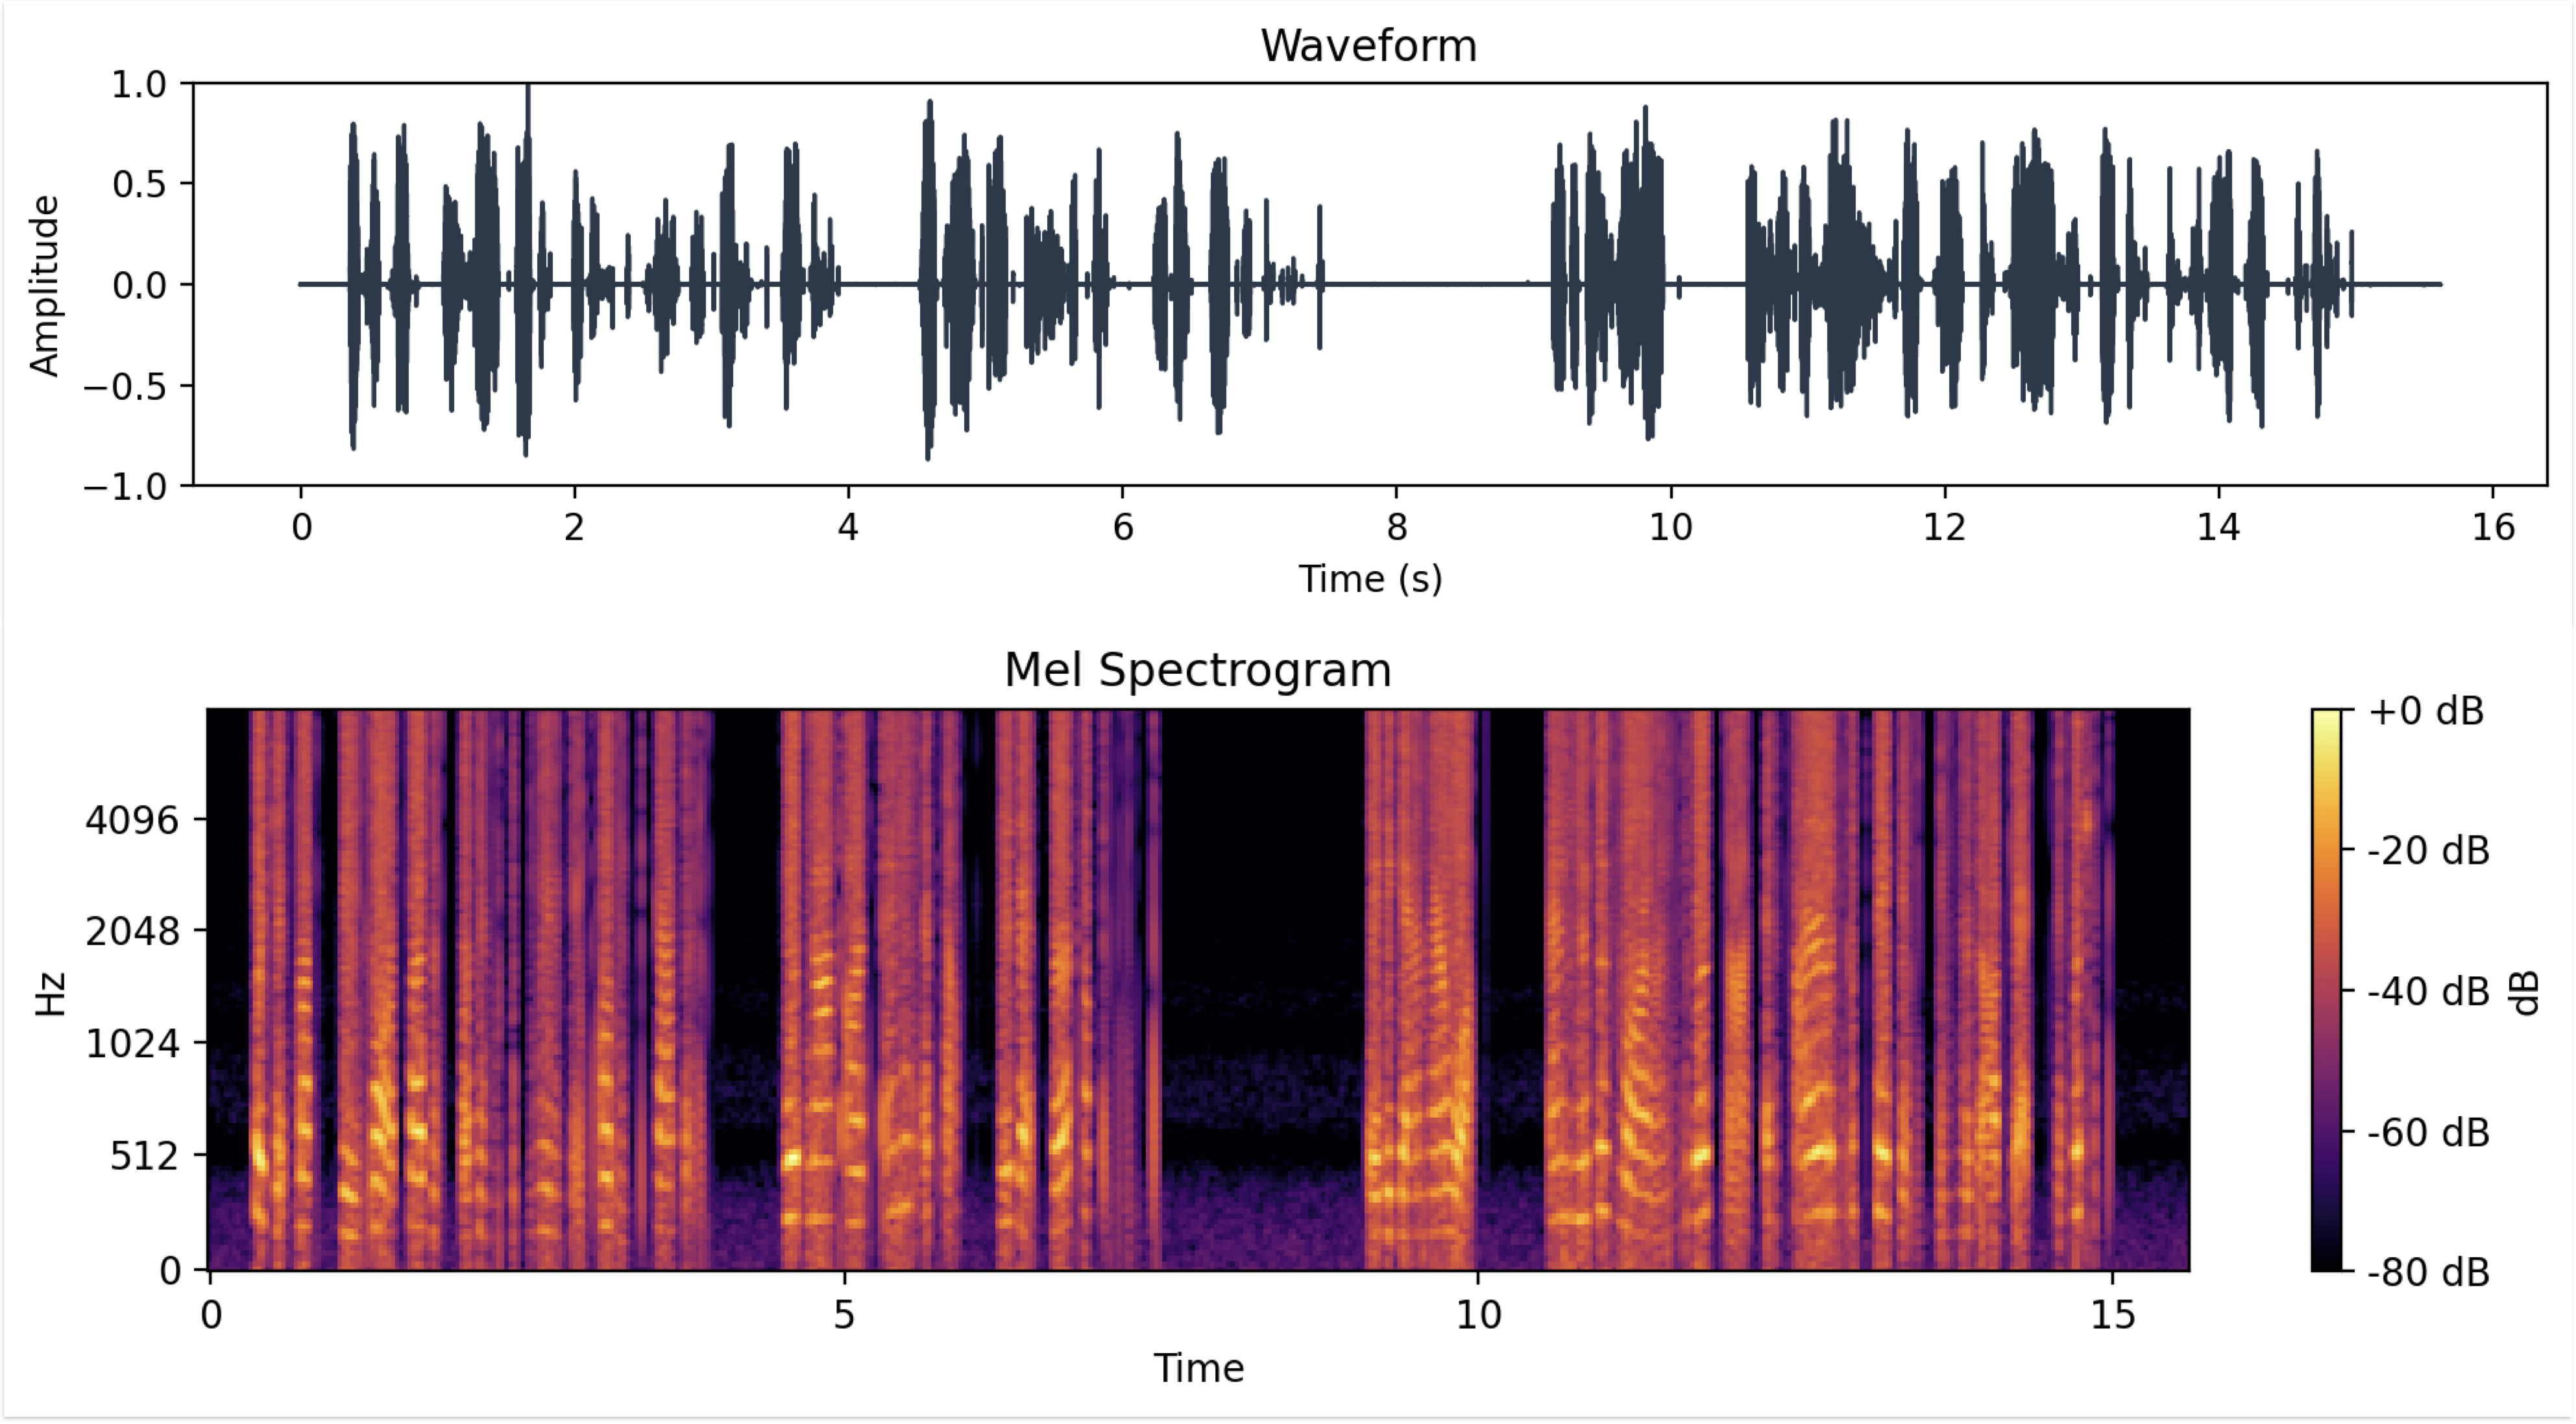
\includegraphics[width=\textwidth]{figures/snr0_w.png}
             \caption{Wiener Filtering}
             \label{fig:five over x}
         \end{subfigure}
            \caption{Speech enhancement results for input signals with an SNR of 0 dB}
            \label{fig:three graphs}
        \vspace{2mm}
    % Finish third block
\end{figure}



\begin{table}[H]
 % Table
    \begin{tabularx}{1\textwidth} { 
      | >{\centering\arraybackslash}X 
      | >{\centering\arraybackslash}X 
      | >{\centering\arraybackslash}X 
      | >{\centering\arraybackslash}X 
      | >{\centering\arraybackslash}X 
      | >{\centering\arraybackslash}X |}
     \hline
      & Noisy & MetricGAN & Wiener & Min-Max & Range\\
     \hline
     PESQ  & 1.06  & 1.12 & 1.05 & 1.05-1.12 & 1.0 - 4.5 \\
     \hline
     STOI  & 0.44  & 0.26 & 0.29 & 0.26-0.44 & 0 - 1 \\
     \hline
     SNR (dB)  & -2.69  & 0.00 & 1.30 & -2.69 - 1.30 & -10 - 30 dB \\
    \hline
    \end{tabularx}
    % Finish table
    \caption{Figure 7.2: In this highly noisy scenario, both MetricGAN and the Wiener filter slightly improve the signal quality compared to the original noisy input. MetricGAN achieves the highest PESQ score (1.12) and matches the input SNR at 0 dB. The Wiener filter slightly surpasses the input with an SNR of 1.30 dB. However, STOI scores are low across all methods, meaning speech remains hard to understand in this very noisy condition. MetricGAN provides a modest advantage in perceptual quality.}
    \label{tab:snr_blocks}
\end{table}

\vspace{2mm}

\begin{figure}[H]
    \centering
         \begin{subfigure}[b]{0.3\textwidth}
             \centering
             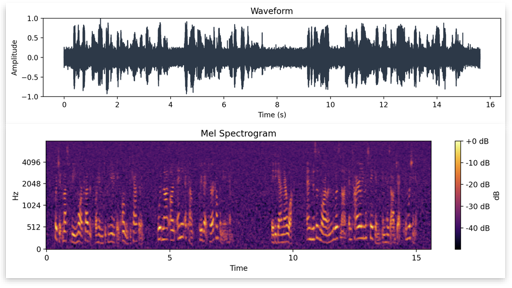
\includegraphics[width=\textwidth]{figures/snr5_o.png}
             \caption{Noisy Speech Signal}
             \label{fig:y equals x}
         \end{subfigure}
         \hfill
         \begin{subfigure}[b]{0.3\textwidth}
             \centering
             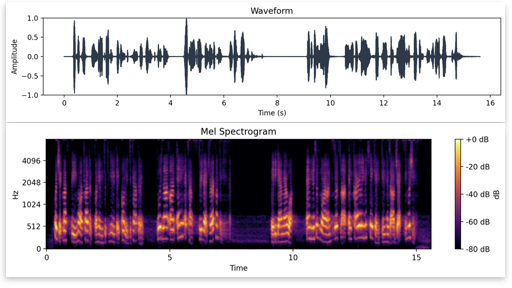
\includegraphics[width=\textwidth]{figures/snr5_e.png}
             \caption{MetricGAN Enhancement}
             \label{fig:three sin x}
         \end{subfigure}
         \hfill
         \begin{subfigure}[b]{0.3\textwidth}
             \centering
             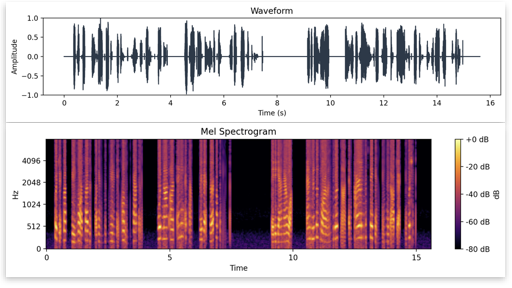
\includegraphics[width=\textwidth]{figures/snr5_w.png}
             \caption{Wiener Filtering}
             \label{fig:five over x}
         \end{subfigure}
            \caption{Speech enhancement results for input signals with an SNR of 5 dB}
            \label{fig:three graphs}
        
    % Finish third block
\end{figure}

\begin{table}[H]
 % Table
    \begin{tabularx}{1\textwidth} { 
      | >{\centering\arraybackslash}X 
      | >{\centering\arraybackslash}X 
      | >{\centering\arraybackslash}X 
      | >{\centering\arraybackslash}X 
      | >{\centering\arraybackslash}X 
      | >{\centering\arraybackslash}X |}
     \hline
      & Noisy & MetricGAN & Wiener & Min-Max & Range\\
     \hline
     PESQ      & 1.12  & 1.91 & 1.07  & 1.07 - 1.91 & 0.5 - 4.5 \\
    \hline
    STOI      & 0.56  & 0.54 & 0.36  & 0.36 - 0.56 & 0 - 1 \\
    \hline
    SNR (dB)  & -0.16 & 2.39 & 1.96  & -0.16 - 2.39 & -10 - 30 dB \\
    \hline
    \end{tabularx}
    % Finish table
    \caption{Figure 7.3: MetricGAN significantly enhances speech quality, raising the PESQ score from 1.12 (noisy input) to 1.91 and improving SNR from –0.16 dB to 2.39 dB. The Wiener filter also improves quality, though less effectively. STOI scores remain similar for both MetricGAN and the noisy input, suggesting limited gains in intelligibility. MetricGAN clearly outperforms the Wiener filter in terms of overall signal clarity and perceptual quality.}
    \label{tab:snr_blocks}
\end{table}

\vspace{2mm}

\begin{figure}[H]
    \centering
         \begin{subfigure}[b]{0.3\textwidth}
             \centering
             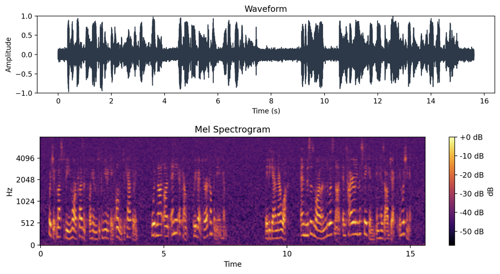
\includegraphics[width=\textwidth]{figures/snr10_o.png}
             \caption{Noisy Speech Signal}
             \label{fig:y equals x}
         \end{subfigure}
         \hfill
         \begin{subfigure}[b]{0.3\textwidth}
             \centering
             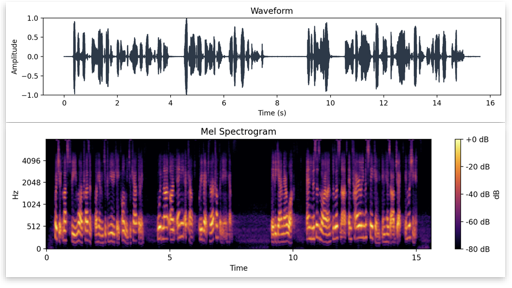
\includegraphics[width=\textwidth]{figures/snr10_e.png}
             \caption{MetricGAN Enhancement}
             \label{fig:three sin x}
         \end{subfigure}
         \hfill
         \begin{subfigure}[b]{0.3\textwidth}
             \centering
             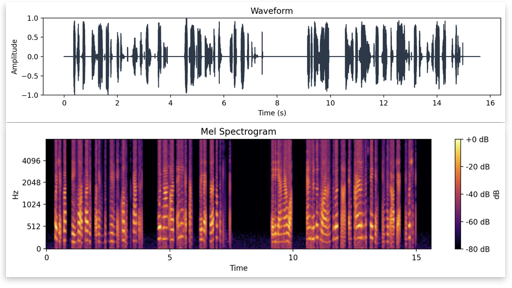
\includegraphics[width=\textwidth]{figures/snr10_w.png}
             \caption{Wiener Filtering}
             \label{fig:five over x}
         \end{subfigure}
            \caption{Speech enhancement results for input signals with an SNR of 10 dB}
            \label{fig:three graphs}
    % Finish third block
\end{figure}

\begin{table}[H]
 % Table
    \begin{tabularx}{1\textwidth} { 
      | >{\centering\arraybackslash}X 
      | >{\centering\arraybackslash}X 
      | >{\centering\arraybackslash}X 
      | >{\centering\arraybackslash}X 
      | >{\centering\arraybackslash}X 
      | >{\centering\arraybackslash}X |}
    \hline
          & Noisy & MetricGAN & Wiener & Min-Max & Range\\
         \hline
        PESQ      & 1.25  & 2.39 & 1.08  & 1.08 - 2.39 & 0.5 - 4.5 \\
        \hline
        STOI      & 0.67  & 0.67 & 0.41  & 0.41 - 0.67 & 0 - 1 \\
        \hline
        SNR (dB)  & 2.90  & 3.81 & 2.62  & 2.62 - 3.81 & -10 - 30 dB \\
        \hline
    \end{tabularx}
    % Finish table
    \caption{Figure 7.4: At 10 dB, both enhancement methods improve the speech signal compared to the noisy input. MetricGAN leads with the highest increase in PESQ (2.39) and SNR (3.81 dB). STOI remains equally good for both MetricGAN and the noisy input (0.67), reflecting good intelligibility, but MetricGAN offers clearer overall audio quality. The Wiener filter improves SNR but falls behind MetricGAN in both PESQ and STOI scores. This highlights MetricGAN's effectiveness at moderate noise levels.}
    \label{tab:snr_blocks}
\end{table}

\vspace{2mm}

\begin{figure}[H]
    \centering
         \begin{subfigure}[b]{0.3\textwidth}
             \centering
             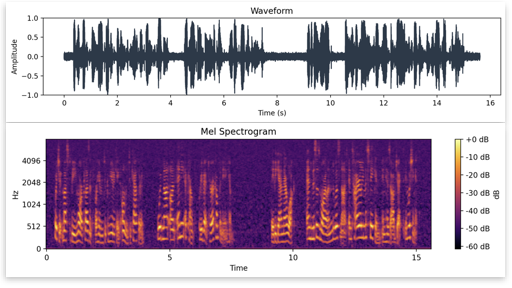
\includegraphics[width=\textwidth]{figures/snr15_o.png}
             \caption{Noisy Speech Signal}
             \label{fig:y equals x}
         \end{subfigure}
         \hfill
         \begin{subfigure}[b]{0.3\textwidth}
             \centering
             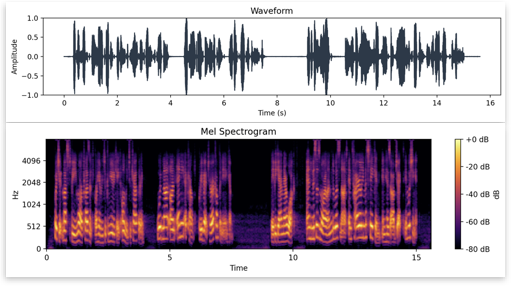
\includegraphics[width=\textwidth]{figures/snr15_e.png}
             \caption{MetricGAN Enhancement}
             \label{fig:three sin x}
         \end{subfigure}
         \hfill
         \begin{subfigure}[b]{0.3\textwidth}
             \centering
             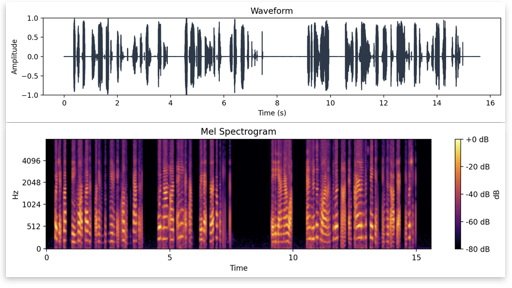
\includegraphics[width=\textwidth]{figures/snr15_w.png}
             \caption{Wiener Filtering}
             \label{fig:five over x}
         \end{subfigure}
            \caption{Speech enhancement results for input signals with an SNR of 15 dB}
            \label{fig:three graphs}
        \vspace{2mm}
    % Finish third block
\end{figure}

\begin{table}[H]
 % Table
    \begin{tabularx}{1\textwidth} { 
      | >{\centering\arraybackslash}X 
      | >{\centering\arraybackslash}X 
      | >{\centering\arraybackslash}X 
      | >{\centering\arraybackslash}X 
      | >{\centering\arraybackslash}X 
      | >{\centering\arraybackslash}X |}
     \hline
      & Noisy & MetricGAN & Wiener & Min-Max & Range\\
     \hline
     PESQ      & 1.51  & 2.79 & 1.09  & 1.09 - 2.79 & 0.5 - 4.5 \\
    \hline
    STOI      & 0.75  & 0.74 & 0.43  & 0.43 - 0.75 & 0 - 1 \\
    \hline
    SNR (dB)  & 6.56  & 5.17 & 3.01  & 3.01 - 6.56 & -10 - 30 dB \\
    \hline
    \end{tabularx}
    % Finish table
    \caption{Figure 7.5: With cleaner inputs, MetricGAN improves the perceptual quality, achieving a PESQ of 2.79 and maintaining high STOI (0.74), slightly better than the noisy input and Wiener filter. Both methods produce clear speech outputs, but MetricGAN consistently excels in perceptual quality and intelligibility, clearly visible in the spectrogram improvements.}
    \label{tab:snr_blocks}
\end{table}

\vspace{2mm}


\begin{figure}[H]
    \centering
         \begin{subfigure}[b]{0.3\textwidth}
             \centering
             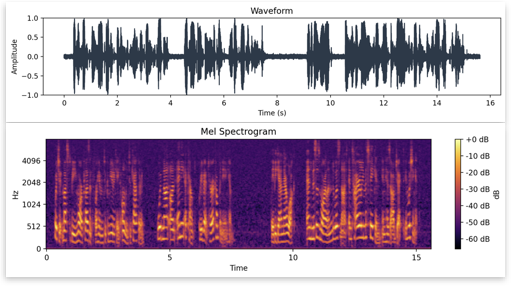
\includegraphics[width=\textwidth]{figures/snr20_o.png}
             \caption{Noisy Speech Signal}
             \label{fig:y equals x}
         \end{subfigure}
         \hfill
         \begin{subfigure}[b]{0.3\textwidth}
             \centering
             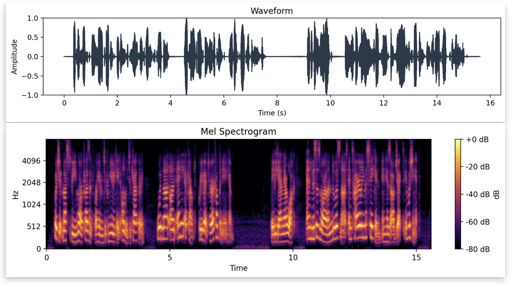
\includegraphics[width=\textwidth]{figures/snr20_e.png}
             \caption{MetricGAN Enhancement}
             \label{fig:three sin x}
         \end{subfigure}
         \hfill
         \begin{subfigure}[b]{0.3\textwidth}
             \centering
             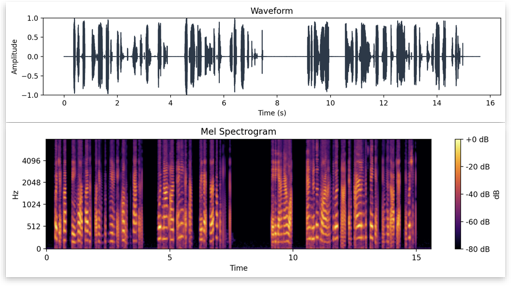
\includegraphics[width=\textwidth]{figures/snr20_w.png}
             \caption{Wiener Filtering}
             \label{fig:five over x}
         \end{subfigure}
            \caption{Speech enhancement results for input signals with an SNR of 20 dB}
            \label{fig:three graphs}
    % Finish third block
\end{figure}

\begin{table}[H]
 % Table
    \begin{tabularx}{1\textwidth} { 
      | >{\centering\arraybackslash}X 
      | >{\centering\arraybackslash}X 
      | >{\centering\arraybackslash}X 
      | >{\centering\arraybackslash}X 
      | >{\centering\arraybackslash}X 
      | >{\centering\arraybackslash}X |}
     \hline
      & Noisy & MetricGAN & Wiener & Min-Max & Range\\
     \hline
     PESQ      & 1.92  & 2.92 & 1.09  & 1.09 - 2.92 & 0.5 - 4.5 \\
    \hline
    STOI      & 0.83  & 0.79 & 0.47  & 0.47 - 0.83 & 0 - 1 \\
    \hline
    SNR (dB)  & 11.16 & 6.35 & 3.12  & 3.12 - 11.16 & -10 - 30 dB \\
    \hline
    \end{tabularx}
    % Finish table
    \caption{Figure 7.6: At 20 dB, the input signal is already quite clean. MetricGAN achieves the highest PESQ score (2.92), but the original noisy input retains slightly higher STOI (0.83) and SNR (11.16 dB). Enhancement improvements are smaller because the audio quality is already high. The Wiener filter only slightly improves or even reduces perceptual quality (PESQ), possibly due to over-smoothing effects. MetricGAN remains a robust and effective choice across various conditions.}
    \label{tab:snr_blocks}
\end{table}


The results show that MetricGAN improves speech quality more effectively than the classical Wiener filter in all tested noise conditions. MetricGAN raises both the clarity and quality of speech, as seen in higher PESQ and SNR scores, and keeps intelligibility high even when noise is strong. These benefits are especially clear when the original audio is very noisy. As the input becomes cleaner, the advantage of using enhancement methods decreases, but MetricGAN still produces consistently good results. Overall, MetricGAN proves to be a reliable and effective method for speech enhancement in a variety of real-world noise scenarios.

